\section{Värmeflöde genom väggar, burspråk och tak}


För att jämföra energiförluster genom en vägg med och utan isolering används
den tidigare beskrivna finita elementmetoden för värmeledningsekvationen i en dimension. Här approximeras
väggen som oändligt lång för enkelhet i beräkningarna. För alla beräkningar har ett tidssteg
på $\Delta t = \unit[500]{s}$ använts med semidiskret MOL.

\begin{figure}[hpbt]
\centering

\subfloat[\label{fig:tempdistapr}
Utomhustemperaturens variation en dag i april.]{
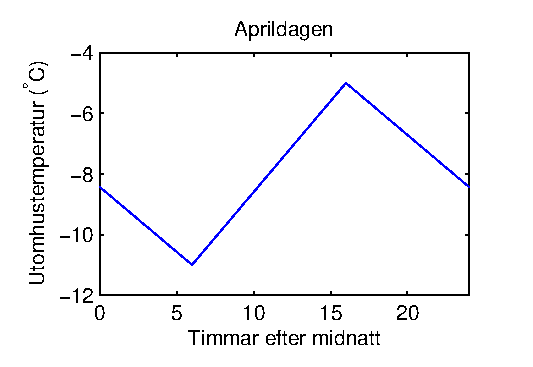
\includegraphics[width=6cm]{images/temperatureapr.eps}}\vspace{1cm}
\subfloat[\label{fig:tempdistdec}
Utomhustemperaturens variation en dag i december.]{
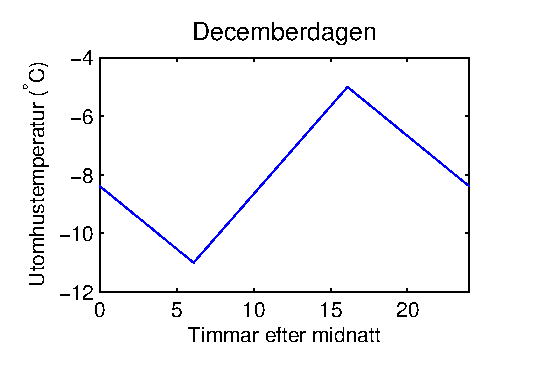
\includegraphics[width=6cm]{images/temperaturedec.eps}
}

\caption{\label{fig:temperaturedist} Utomhustemperaturens variation under standarddagarna motsvarande mitten av april samt den sista december som varierar mellan $\unit[6]{^\circ C}$ på natten och $\unit[9]{^\circ C}$ på dagen respektive $\unit[-11]{^\circ C}$ på natten och $\unit[-5]{^\circ C}$ på dagen.
}
\end{figure}


I detta försök antas att en perfekt värmeanläggning
existerar så att temperaturen inomhus hålls till konstanta $\unit[20]{^\circ C}$. Efter detta specificeras energiflödet
från utsidan av väggen genom vilka energiflöden som strömmar till väggen. Dessa är svartkroppsstrålning, solinstrålning
samt konvektion. Beräkningarna är sedan genomförda med solinstrålningsdata från en solig och en molning decemberdag samt
en solig aprildag och en molning aprildag. Solens position och mängden svartkroppsstrålning är beräknade enligt avsnitt
\ref{sec:sunthroughwindows} och avsnitt \ref{sec:blackbody}.
Konvektionsparametern är sedan satt till $h=\unit[6,19]{Wm^{-2}K^{-1}}$ för aprildagen vilket motsvarar helt vindstilla.
För decemberdagen sattes konvektionsparametern till $h=\unit{35}{Wm^{-2}K^{-1}}$ vilket motsvarar en decemberdag med en vindhastighet på $v=\unit[7]{ms^{-1}}$ parallellt
med ytan.
Under aprildagen varierade temperaturen linjärt från $T=\unit[6]{^\circ C}$ klockan 06:00 och $T=\unit[9]{^\circ C}$ 16:00 vilket kan ses i figur \ref{fig:tempdistapr}.
Samma värden för decemberdagen är $T = \unit[-11]{^\circ C}$ 06:00 respektive $T=\unit[-5]{^\circ C}$ 16:00 vilket kan ses i figur \ref{fig:tempdistdec}.

Problemet har sedan satts upp för två olika väggar. Först en som enbart innehåller $\unit[0,5]{m}$ tegel med
en värmeledningsförmåga på $k = \unit[0,6]{Wm^{-1}K^{-1}}$ och volymetrisk värmekapacitet på
$c_{p}\rho = \unit[1,154]{MJm^{-3}}$. Den andra väggen har först samma tegellager men
har sedan tilläggsisolerats på utsidan med $\unit[0,1]{m}$ mineralull. Mineralullen har värmeledningsförmåga på
$k = \unit[5,2\cdot 10^{-7}]{Wm^{-1}K^{-1}}$ och volymetrisk värmekapacitet på
$c_{p}\rho = \unit[58,8]{kJ m^{-3}}$. \cite{kandidatarbete2010}\cite{engineeringtoolboxdensity}\cite{bkvthermal}\cite{engineeringtoolboxspecificheat}

Under experimentens gång så har ett godtyckligt initialvärde valts för att sedan vänta tills
lösningen stabiliserat sig för att då utläsa energiåtgången. Derivatan på insidan har slutligen beräknats
och använts för att beräkna kyleffekten genom Fouriers värmelag.

Vidare har väggarnas stegsvar undersökts. Experimentet startades med att väggarna var i jämvikt med en utomhustemperatur på $T = \unit[0]{^\circ C}$ sedan steg till $T = \unit[10]{^\circ C}$ vid tiden $t=0$. Konvektionsparametern är här satt till
$h = \unit[25]{W m^{-2}K^{-1}}$ vilket motsvarar en vind på ungefär 
$v = \unit[5]{ms^{-1}}$ parallellt med väggens yta. Genom att beräkna den momentana kyleffekten för varje tidssteg kunde väggarnas tröghet studeras.

För burspråk och tak har ungefär samma metod som för väggen följts, med simuleringar motsvarande soliga och
molniga december- respektive aprildagar. Samma temperaturförändringar som beskrivits ovan har använts för
respektive fall. Skillnaderna ligger i vilka material de olika byggnadsdelarna är uppbyggda av.
Burspråket har simulerats med materialen och tjocklekarna angivna för burspråken i figur \ref{fig:bursprak}.
Kopparens värmeledningsförmåga har satts till $k=\unit[401]{Wm^{-1}K^{-1}}$, koppars volymetriska värmekapacitet till $\rho c_p = \unit[3,49]{MJm^{-3}}$, spånskivans värmeledningsförmåga $k = \unit[0.5]{Wm^{-1}K^{-1}}$, spånskivans volymetriska
värmekapacitet $\rho c_p = \unit[1,3]{MJm^{-3}}$, putsets värmeledningsförmåga $k = \unit[0.25]{Wm^{-1}K^{-1}}$, puts volymetriska
värmekapacitet $\rho c_p = \unit[872]{kJm^{-3}}$ och slutligen mineralullens värden
enligt tidigare.
\cite{engineeringcom}\cite{kandidatarbete2010}\cite{engineeringtoolboxthermalconductivity}\cite{engineeringtoolboxspecificheat}

Taket är uppbyggt enligt figur \ref{fig:taket} och består av omkring tre centimeter tegelpannor med materialkonstanterna $k = \unit[0,85]{Wm^{-1}K^{-1}}$ och $c_p\rho = \unit[920\cdot 1900]{Jm^{-3}}$.
\emph{\color{red} Källor} och 21 centimeter mineralull. Den lilla påverkan som gipset medför har försummats. Övriga skillnader mellan beräkningar på värmeflödet genom taket och väggarna härstammar från det faktum att solstrålningens normalprojektion är annorlunda på taket jämfört med vertikala ytor, något som tagits med i beräkningarna. Dessutom blir denna projektion olika beroende på om man betraktar nordsidan eller sydsidan av taket, varför dessa två delar har simulerats separat för de soliga dagarna. De molniga dagarna har däremot antagandet att en femtedel av maximala solintensiteten infaller på samtliga ytor, då all strålning kan antas vara indirekt.


